\documentclass[a4paper,11pt,pdf]{../templates/pacmanreport}

%%=== Aditional packages


%%=== Local definitions
\graphicspath{{images/}{../shared_images/}}

%% ================================
%% PROJECT INFO 

\project{}
\projectid{FP7-IST-60918}
\projectstart{1 March 2013}
\duration{36}

%% ================================
%% DELIVERABLE INFO 

\title{Planning Active Information Gathering for Haptic and Vision}
\deliverableid{DR 3.2}
\author{C. Zito, C. Rosales, F. Spinelli, A. Rietzler, E. Arruda, J. L. Wyatt}
\address{School of Computer Science, University of Birmingham}
\email{claudio.zito.81@gmail.com}
\headertitle{Active Information Gathering}
\headerauthor{C. Zito}

\duedate{2015-02-27}
\submissiondate{2015-02-27}
\leadpartner{BHAM}
\revision{draft}
\disseminationlevel{PU}


%% UNCOMMENT: to get the logo; if you've copied this file to a directory yearX/wpY/ then this should work
\reportlogo{pacmanlogo}


\begin{document}

\maketitle

\begin{abstract}
\noindent 
This report describes activities related to the development of planning algorithms for actively gathering information for object of unknown shape. 
This report presents the efforts on the definition of information theoretic measures for uncertainty about shape as well as modelling of incomplete surfaces. 
It also describes how to integrate low-level controllers, developed on Task 3.1, to plan haptic exploration strategies for a bi-manual robot which holds in one 
hand an unknown object and is capable of tracing the object's surface with a sensorised finger. 
Further, work is introduced, where we describe a novel method for planning actions to actively gain 
information about an object's pose belief via proprioceptive sensing using an adaptive robotic hand.
\end{abstract}


\vspace{.2em}
\hrule

\footnotesize

\tableofcontents

\normalsize

\newpage

\section*{Executive Summary}

This report describes the activities within the PaCMan consortium to define methodologies for \emph{active information gathering}.
The material included in this report presents results on reactive control strategies for haptic exploration developed in Task 3.1 (M 1-18) 
as well as results on planning and execution of active visual information gathering developed in Task 3.3 (M 1-36).

\section*{Role of active information gathering in PaCMan}

This deliverable presents the achievements of the consortium in the development of new strategies for planning of active information gathering actions. 

\section*{Contribution to the PaCMan scenario}

Robot grasping is typically affected by uncertainty associated to the location of the object to be grasped as well as its shape. 
A robot could gather information either by i) touching the object or ii) visually observing it from different point of views. 
This report presents three approaches that enable a robot to reason about such uncertainties and to plan the best-next action to maximise the information gain.

\newpage

\section{Tasks, objectives, results}

\subsection{Planned work}

This deliverable addresses the work developed in Task 3.2 and Task 3.3.
In particular, the development of planning active strategies for information gathering through both vision and 
haptic exploration of unknown objects. 
This includes using vision and haptic clues to build probabilistic models of the object to be manipulated.   

\subsection{Actual work performed}

The work we have done can be divided in three sections: i) tactile exploration of unknown objects; ii) object localisation through proprioceptive information gain; and iii) active gaze control planning. The next sections describe each of these approaches and summarise their contributions.

\subsection{Tactile exploration}

This task addresses the problem of planning and execute active information gathering for objects of unknown shape, as formulated in Task 3.3. Our solution employs a Gaussian Process (GP) for estimating an implicitly-defined function as well as provide a measurement of the uncertainty on the estimated surface. The approximating function can be considered as the 0-levelset of the surface of the object to be manipulated, it comes handy to interpret it as a manifold and to build on recent developments on sample-based techniques for manifold explorations, e.g.~\cite{Jaillet2013Path}. We extend such algorithms to define the next-best exploration action to minimise the reduction of shape uncertainty. 

The work in~\cite{Dragiev2011Gaussian} is one of the first attempt to employ GP for implicit surfaces for representing shapes in tasks as robotic grasping. However, the authors rely only on the MAP estimation of the surface (its mean) without exploiting the model uncertainty. The same authors in~\cite{Dragiev2013Uncertainty} extended their previous work to formulate a way to make inference from the GP to prefer regions on the model with particular certainty level and introduce the concept of explore-grasp and exploit grasp primitives. 

Our proposed solution has several advantages: i) it implicitly defines the unknown shape in a probabilistic model, ii) integrates visual and haptic information in its model to refine its predictions and iii) constructs paths on the object's surface that a robot equipped with a sensorised finger can follow in order to gather haptic information. 
The algorithm is demonstrated in simulation and on a real robotic platform (Vito) where a bi-manual robot holds an unknown object in its hand and it is capable of tracing the object surface with the other arm equipped with a F/T sensor.
%do we have a paper to cite about the probe finger?

The experimental results show that our framework can learn the object shape and yields to better models with a reduced number of exploration actions.

\subsection{Proprioceptive information gain using adaptive hands for pose refinement}
%Connecting with Task description..

This work solves the problem of reducing the uncertainty in the pose of an object by actively gathering information via proprioception.
Our proprioceptive measurements are integrated into an occupancy grid, which is subsequently used to update the pose belief.
In that sense, our occupancy grid also represents the object's shape. 
In contrast to explicitly modelling the uncertainty of the object via object model pose hypotheses, the occupancy grid is suited to 
represent unknown shape. Therefore, our work is easily extendable to gain shape information of unknown objects and thus touches the core of Task 3.2.

%related work
In the case of selecting actions based on tactile information gain, robot-environment interaction has to be taken into account. 
Hebert et. al. \cite{Hebert2013} have introduced a method to select the next best touching action to localise the 3D object position or other object model parameters.
Similar to our work they choose an action from a set of predefined candidate actions. 
To update the belief over object parameters they use a combined measurement model that is based on both binary contact detection and tactile sensors.  
In contrast, we use only proprioceptive measurements of occupancy, which enables us to gain information
when we do not interact with the object at all.

Recent work from Wong et. al. \cite{Lawson2016Not} combines the occupancy grid representation and object-based representations like belief over an object's pose and identity 
in a general way. They illustrate a motivating example where they use contact-free proprioceptive measurements of an robot arm to update an 
occupancy grid and subsequently are able to distinguish between two different objects. 
We extend there work in the sense that we also gain information purely by proprioception, but in contrast we provide an automated way to compute 
a robot action to do so.
%Our solutution
We  solve this problem by representing robot actions by manually defining a set of action primitives comprised of end-effector translations direction and
open close states for the robotic hand. In the planning step reachable end-effector poses are searched and the associated actions are ranked 
by expected information gain.
The actions are executed and the occupancy grid and subsequently the pose belief are updated depending on the proprioceptive measurements of the robotic hand.
%Whats good about our algorithms
The novelty of algorithm is that it uses proprioception instead of tactile contact. Because we model the probability of touching the object 
given the current progress of the action and because our measurements are purely proprioceptive, we can influence that we touch the object at all but still 
gain information about its pose belief. This might be helpful in cases of exploring lightweight objects that move easily and do not 
generate measurable forces at touching sensors.
Another promised advantage of our method is the use of an adaptive hand. This should lead to a higher amount of 
relevant proprioceptive measurements close to object surfaces while not moving the object due to the adaptability.
%First results
In our technical report we show the theoretical background of our proposed method and intermediate results on implementation. 
So far we implemented the occupancy aware pose distribution sampling, computation of the occupancy grid posterior and the definition of the action primitives.
In the next steps we want to we want to compare the effectiveness of the different action primitives in refining the pose belief in scenarios with objects 
having different masses and sizes and different levels of occlusion. 

\subsection{Active gaze control planning}

Grasping on novel objects relies on the quality and completeness of the shape reconstruction through noisy perception. Given an active vision system, we would like to minimise the number of views taken, while maximising grasping reliability. Active vision, or more generally active perception, is defined as the study of modelling, planning and control strategies for perception when the sensor can be actively moved \cite{Bajcsy88activeperception}. In the context of manipulation, researchers have focused on devising strategies for view selection based on recovery of the full shape of the object to be grasped \cite{krainin2011autonomous,Chen2011IJRoboticRes}. For most practical manipulation purposes, however, full object reconstruction is too costly or simply infeasible. It is also typically redundant, since most of the time only a limited portion of the object surface is in contact during a grasp  \cite{kopicki2015}. 

At the root of the difficulties is a chicken and egg problem. On the one hand, given that the initial point cloud can be highly incomplete, it is hard to plan a reliable grasp to begin with. On the other hand if we knew the likely planned grasp then we could direct gaze more efficiently. In this paper we solve this problem by employing a grasp planner that can generate grasps for novel objects in the face of fragmentary reconstructions. We use grasp candidates to guide active vision, and the results of active vision to refine grasp planning.

In our scenario, the robot begins by taking a single view from a fixed location of the scene. A depth camera is used, and this gives an incomplete point cloud. A dexterous grasp planning algorithm is then run, which generates a large number of candidate grasps on the partial point cloud for the object. These grasps will typically assume the existence of graspable surfaces on both sides of the surface defined by the point cloud. The predicted contact locations are then used to drive the next view. The next view is chosen to maximise the quality of the point cloud at the planned contact locations. If a grasp cannot be found, we employ information gain view planning, using 3D occupancy map. Once the quality of the relevant surface reconstruction is sufficiently high, or a limit on the number of views is reached, the grasp is fixed. Then a second phase of active vision aims to verify a safe path to the grasp location. To achieve this we again use the 3D occupancy map. This is used to calculate the probability of a collision free trajectory. Active views for safety are driven to reduce the average entropy in cells through which the candidate reach-to-grasp trajectory passes. This ensures a safe grasp.

%\subsection{Relation to the state-of-the-art}

%The following paragraph discusses work related to our work about proprioceptive information gain for pose refinement.



\bibliographystyle{ieeetr}
\bibliography{../shared_bibliography/abbreviations,./bibliography/DR32}

\newpage

\appendix
\section{Annexes} 

% template for annexes
%\subsection{Book chapter/Article/Technical Report: \em TITLE}
%\begin{description}
%    \item[Authors] 
%    \item[Info] % UNDER REVIEW / IN PRESS / ACCEPTED FOR PUBLICATION (PROVIDE WHERE) / PUBLISHED AND AVAILABLE ONLINE (PROVIDE DOI)
%    \item[Abstract]
%    \item [Relation with the deliverable] 
%    \item[Attachment] %if so, e.g. (following pages until next annex) or The article can be downloaded at the DOI link above, hence no attachment is provided
%\end{description}
% attach your PDF(s) if required, pusblished and online available documents do not require it if you provide the doi (only doi are permitted)
%\includepdf[pages=-]{./attachedPapers/YOURFILE.pdf

\subsection{Journal paper: \em GPAtlasRRT: A tactile exploration strategy for novel object shape modeling}
\begin{description}
    \item[Authors] Carlos J. Rosales, Claudio Zito, Federico Spinelli, Marco Gabiccini and Jeremy L. Wyatt
    \item[Info] UNDER REVIEW %/ IN PRESS / ACCEPTED FOR PUBLICATION (PROVIDE WHERE) / PUBLISHED AND AVAILABLE ONLINE (PROVIDE DOI)
    \item[Abstract] Information on object shape is a fundamental parameter for robot-object interaction to be successful. However, incomplete perception and noisy measurements impede obtaining accurate models of novel objects. Especially when vision and touch simultaneously are envisioned for learning object models, a representation able to incorporate prior shape knowledge and heterogeneous uncertain sensor feedback is paramount to fusing them in a coherent way. Moreover, by embed- ding a notion of uncertainty in shape representation allows to more effectively bias the active search for new tactile cues. In this work, we use a Gaussian Process (GP) as such representation. Then, using the fact that the 0-levelset of the GP � the surface of the object � is an implicitly defined manifold, we borrow the AtlasRRT algorithm concept to simultaneously: (i) build an atlas via continuation methods that locally parameterises the object and that is used to select the next- best touch, and (ii) use an RRT-like strategy to devise directions for the expansion of the atlas to trade completeness in the exploration for efficiency. We integrate this strategy in a framework for iterative learning the object shape and implement a tactile exploration scenario in the bi-manual setting of our Vito robot. The experimental results confirm that the devised strategy yields better models compared to a naive strategy, and does it with a reduced number of touches.
    
    \item [Relation with the deliverable] This work addresses the problem of planning and execute active haptic information gathering for unfamiliar object (Task 3.2).
    \item[Attachment] (following pages) %if so, e.g. (following pages until next annex) or The article can be downloaded at the DOI link above, hence no attachment is provided
\end{description}
% attach your PDF(s) if required, pusblished and online available documents do not require it if you provide the doi (only doi are permitted)
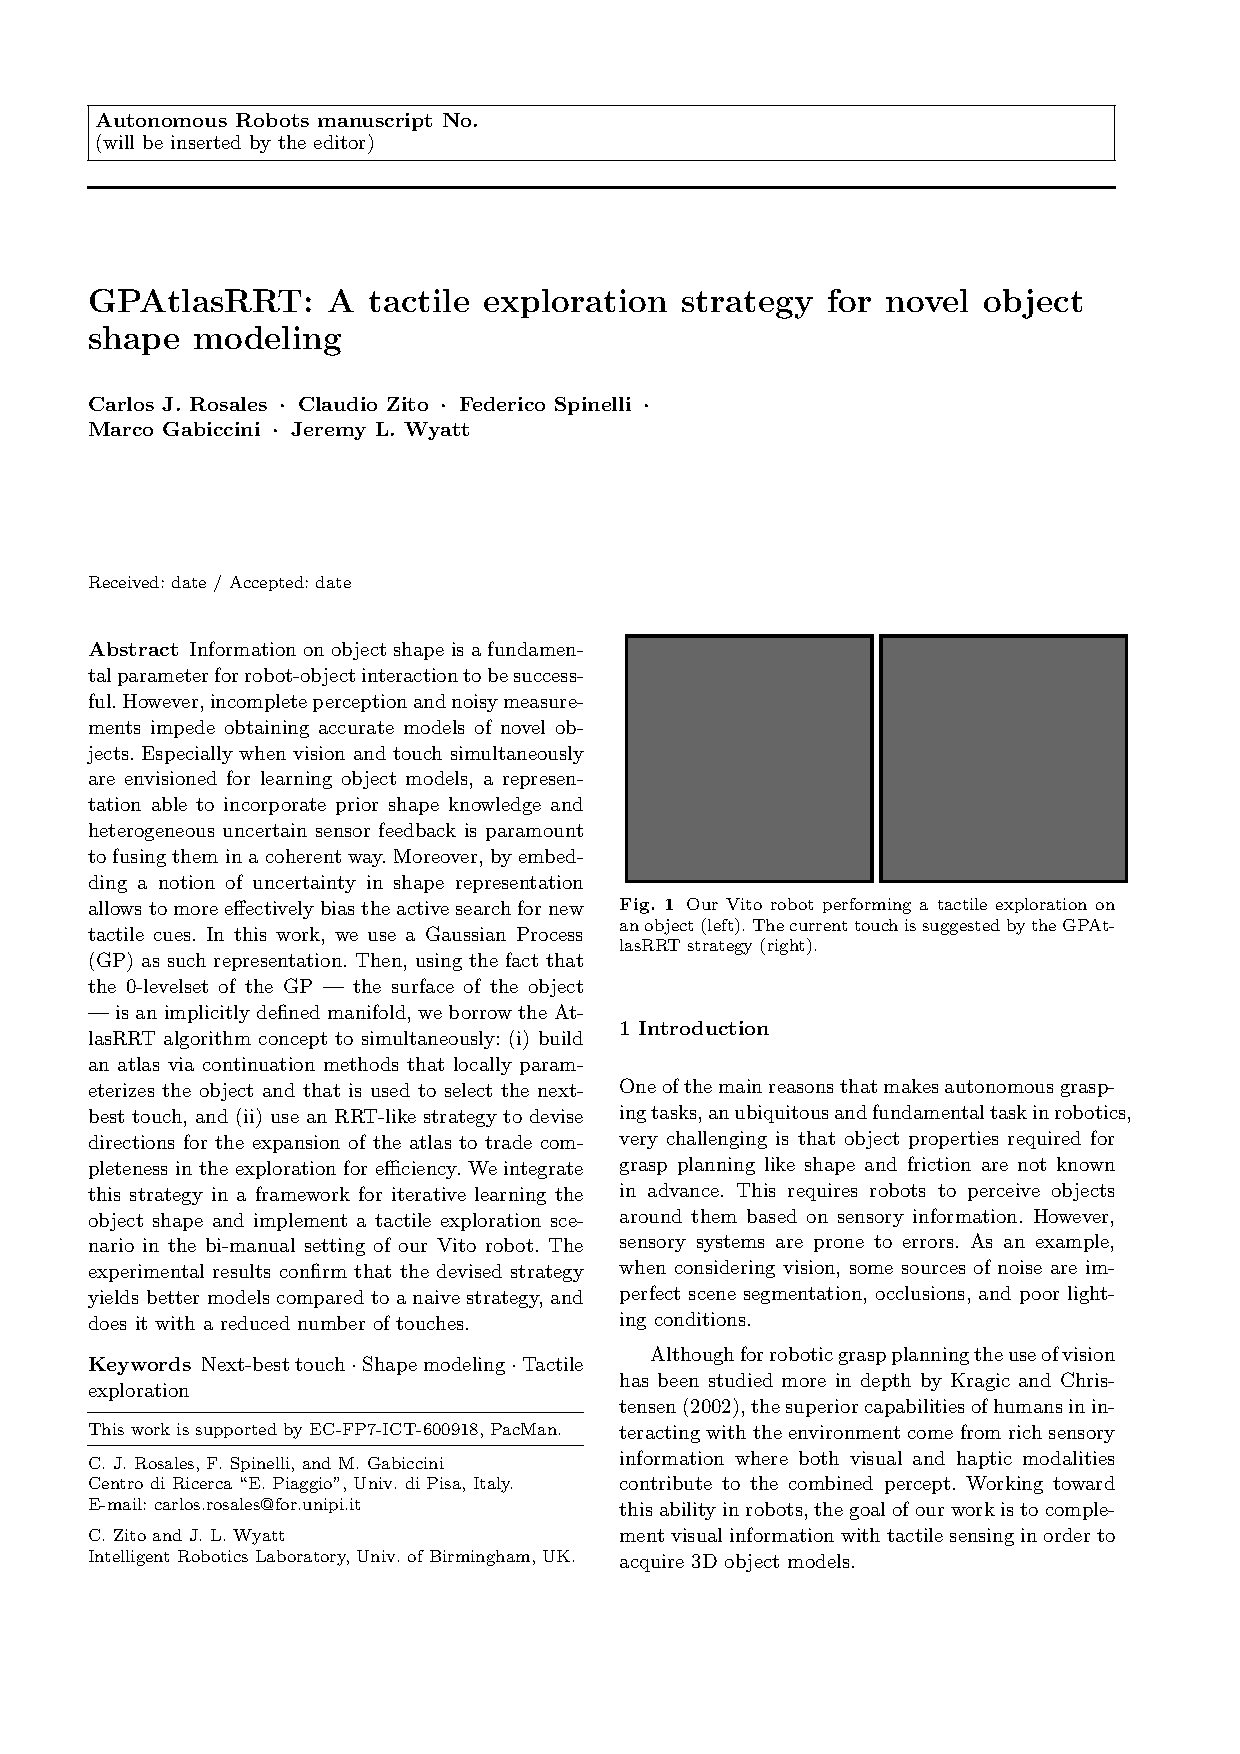
\includepdf[pages=-]{./attachedPapers/rosales_auro_2016.pdf}

%%%%%%%%%%%%%%%%%%%%%%%%%%%%%%%%%%%%%%%%%%%%%%%%%%%%%%%%%%%%%%%%%%%%%%%%%%%%%%%%%

\subsection{Technical Report: \em The Next Best Touch or Non-Touch:
Object Pose Estimation via Sculpting with Compliant Hands}
\begin{description}
    \item[Authors] Alexander Rietzler, Carlos J. Rosales, Marco Gabiccini and Justus Piater
    \item[Info] Paper draft% UNDER REVIEW / IN PRESS / ACCEPTED FOR PUBLICATION (PROVIDE WHERE) / PUBLISHED AND AVAILABLE ONLINE (PROVIDE DOI)
    \item[Abstract] Many robotic tasks rely on the ability of a vision system to accurately estimate the 6 dimensional pose of objects in a scene.
In many cases a single vision sensor does not provide sufficient information to discriminate a single correct
pose of an object. This work solves the problem of refining the pose distribution 
of an object solely via proprioceptive sensing of occupancy.
Our main novel contribution is an algorithm that plans a robot arm-hand trajectory such that 
information gathered about the object pose belief is maximized while at the same time impact on the object is minimized. 
This may result in actions that do not make contact with the object at all.
Impact on the object is further reduced by using a compliant robotic hand.
In this report our the theoretical foundations of our ongoing work are presented and intermediate results are shown. %on occupancy aware pose belief sampling and the definition of the action primitives are shown.

    \item [Relation with the deliverable] This report reports work done under\\ Task~3.2 by introducing a method for reducing an object's pose uncertainty by performing proprioceptive information
    gathering actions.
    \item[Attachment] (following pages) %if so, e.g. (following pages until next annex) or The article can be downloaded at the DOI link above, hence no attachment is provided
\end{description}
% attach your PDF(s) if required, pusblished and online available documents do not require it if you provide the doi (only doi are permitted)
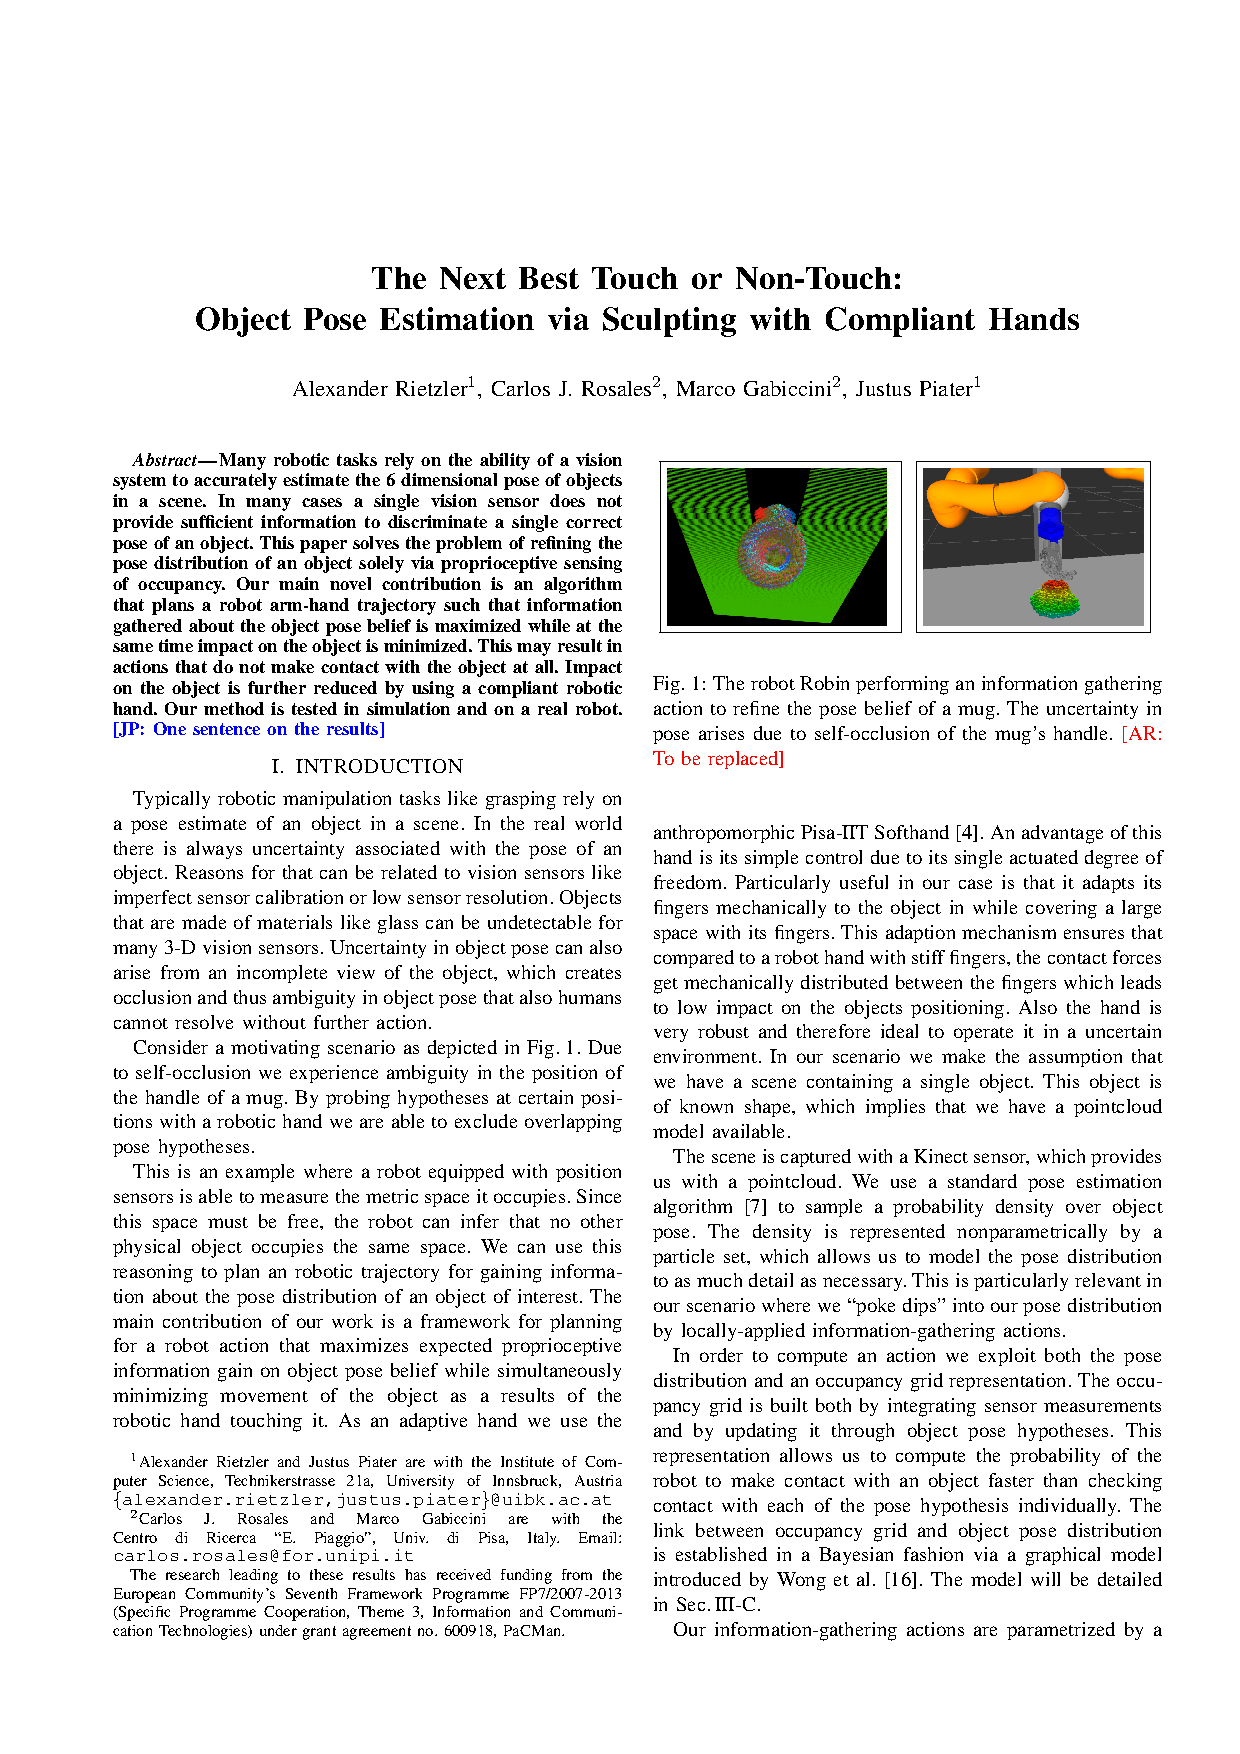
\includepdf[pages=-]{./attachedPapers/iros_draft_rietzleretal.pdf}

%%%%%%%%%%%%%%%%%%%%%%%%%%%%%%%%%%%%%%%%%%%%%%%%%%%%%%%%%%%%%%%%%%%%%%%%%%%%%%%%%

\subsection{Conference paper: \em Active vision for dexterous grasping of novel objects}
\begin{description}
    \item[Authors] Ermano Arruda, Marek Kopicki and Jeremy L. Wyatt
    \item[Info] UNDER REVIEW %/ IN PRESS / ACCEPTED FOR PUBLICATION (PROVIDE WHERE) / PUBLISHED AND AVAILABLE ONLINE (PROVIDE DOI)
    \item[Abstract] How should a robot direct active vision so as to ensure reliable grasping? We answer this question for the case of dexterous grasping of unfamiliar objects. When an object is unfamiliar, much of its shape is by definition unknown. An initial view will recover only some surfaces, leaving most of the object�s surface unmodelled, and also leaving shadow regions which may or may not contain obstacles. These two features make it difficult both to select reliable grasps, and to plan safe reach-to-grasp trajectories. Grasps typically fail in one of two ways, either unmodelled objects in the scene cause collisions, or object reconstruction is insufficient to ensure that the grasp points provide a stable force closure. These problems can be solved more easily if active sensing is guided by the anticipated actions. Our approach has three stages. First, we take a single view and generate candidate grasps from the resulting partial object reconstruction. Second, we drive active vision to maximise surface reconstruction quality around the planned contact points. During this phase the anticipated grasp is continually refined. Third, we direct gaze to unmodelled regions that will affect the planned reach to grasp trajectory, so as to confirm that this trajectory is safe. We show, on a dexterous manipulator with camera on wrist, that our approach (85.7% success rate) outperforms a randomised algorithm (48% success rate).
    \item [Relation with the deliverable] This work addresses the problem of planning and execute active visual information gathering for unfamiliar object (Task 3.3).
    \item[Attachment] (following pages) %if so, e.g. (following pages until next annex) or The article can be downloaded at the DOI link above, hence no attachment is provided
\end{description}
% attach your PDF(s) if required, pusblished and online available documents do not require it if you provide the doi (only doi are permitted)
\includepdf[pages=-]{./attachedPapers/arruda_iros_2016.pdf}

\end{document}
